\documentclass{article}
\usepackage[utf8]{inputenc}

\usepackage{mathtools}
\usepackage{hyperref}
\hypersetup{
    colorlinks=true,
    linkcolor=blue,
    filecolor=magenta,      
    urlcolor=cyan,
}

\title{Actividad 3}
\author{Miguel Terán}
\date{1 de septiembre de 2021}

\begin{document}




\maketitle
\section{Medición de tiempos de procesado}


Para esta actividad se procedió a ejecutar el programa \textit{trap} con diferentes números de procesos. Los \textit{nodos} que se utilizaron fueron: \textit{cero, uno, tres, cinco, seis, siete, ocho, nueve, diez, once, doce, trece, catorce} y \textit{quince}, es decir, solo se utilizaron $14$ nodos. Ello, debido a fallas técnicas presentadas a la hora de realizar las mediciones. Los nodos utilizados permitió ejecutar el programa hasta con un número de procesos máximo de $56$.

En la figura \ref{fig1} se puede observar los datos recopilados para los tiempos \textit{real}, \textit{user} y \textit{sys}, los cuales son el producto de un promedio de tres series de mediciones para cada categoría de tiempo. Se puede apreciar en la figura que los datos muestran un comportamiento lineal con pendiente positiva. Esto, significa que el tiempo de procesado del programa en ejecución aumenta con respecto al número de procesos.

En la figura \ref{fig2} se muestra un promedio de los tiempos \textit{real}, \textit{user} y \textit{sys}. Esto, para tener una perspectiva general del tiempo de procesado del programa ejecutado en cuestión. En esta gráfica se puede observar dos regiones. La primera región que está entre $1$ y $10$ número de procesos, se puede observar un comportamiento lineal, pero con una pendiente muy pronunciada. Por otro lado, en la segunda región que está entre $10$ y $56$ se observa un comportamiento relativamente estable, pero con un patrón de crecimiento en el tiempo a medida que el número de procesos aumenta. 

\begin{figure}[h]
    \centering
    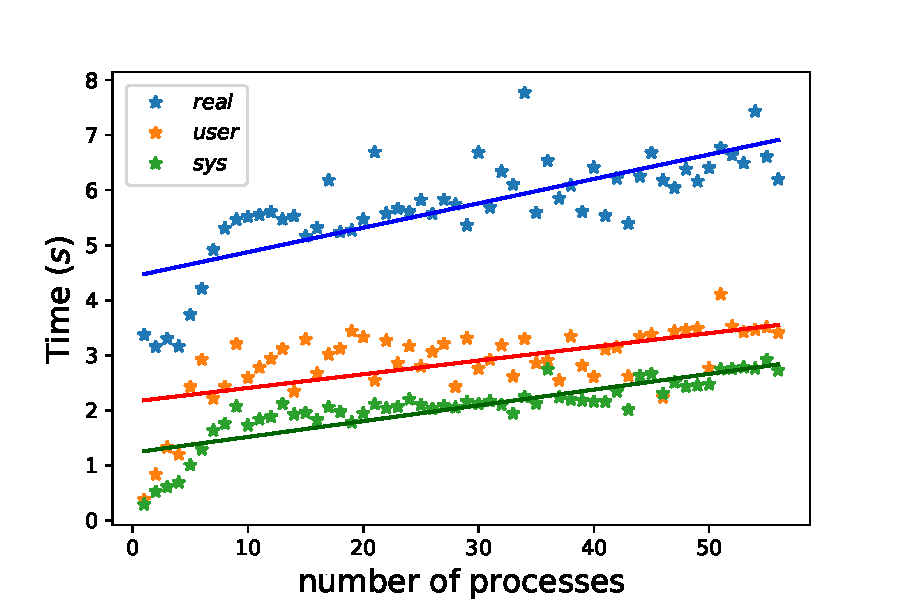
\includegraphics[width=4in]{timeProcesses.pdf}
    \caption{Se muestra los datos correspondientes a los tiempos \textit{real}, \textit{user} y \textit{sys}. Asimismo, en la gráfica se muestra los ajustes lineales correspondientes para cada conjunto de datos. La línea azul corresponde a la ecuación: $t_1=0.044*np + 4.431$, la línea roja corresponde a la ecuación: $t_2=0.024*np + 2.159$ y la línea verde corresponde a la ecuación: $t_3 = 0.028*np + 1.232$.} \label{fig1}
\end{figure}

\begin{figure}[h]
    \centering
    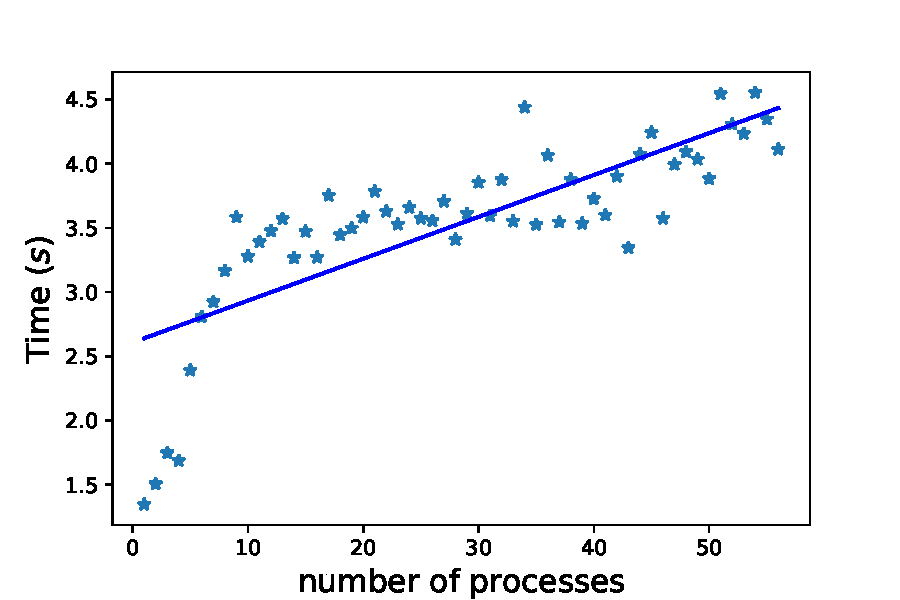
\includegraphics[width=4in]{timeProcesses2.pdf}
    \caption{Se muestra un promedio de los tiempos \textit{real}, \textit{user} y \textit{sys}. La línea azul corresponde a la ecuación: $t =0.032*np + 2.607$. } \label{fig2}
\end{figure}

\section{Conclusiones}
En esta actividad se pudo observar que aunque el programa \textit{trap} es compatible con la programación en paralelo, para este caso no es viable bajo los parámetros usados. El tiempo de procesado aumentó a medida que se utilizaron más procesadores. Ello, se puede adjudicar posiblemente al costo de tiempo de la comunicación entre los \textit{nodos}. 

\end{document}

